\documentclass[12pt,a4paper]{report}
\usepackage[margin=2.5cm]{geometry}
\usepackage[magyar]{babel}

% magyar nyelv tamogatas
\usepackage{t1enc}
\usepackage[T1]{fontenc}
\usepackage[utf8]{inputenc}

% A formai kovetelmenyekben megkövetelt Times betűtípus hasznalata:
\usepackage{times}

\usepackage{setspace}
\usepackage{listings,multicol}
\usepackage{xcolor}
\usepackage{textcomp}
\usepackage{enumitem}
\usepackage{booktabs}
\usepackage[unicode,hidelinks]{hyperref}
\usepackage{footnote}
\usepackage{ifthen}

% Törölhető package
\usepackage{lipsum}

% TODO csomag, amivel jól észrevehető todokat hagyhatunk a dolgozatban
\usepackage{todonotes}
% Inline TODO
\newcommand{\todoi}[1]{\todo[inline]{\textbf{TODO:} #1}}

% egyedi lablec
\usepackage{fancyhdr}
\usepackage{graphicx}
\graphicspath{{fig/}}

% Kódrészletes színezése
\definecolor{lightgray}{rgb}{.9,.9,.9}
\definecolor{darkgray}{rgb}{.4,.4,.4}
\definecolor{purple}{rgb}{0.65, 0.12, 0.82}

\lstdefinelanguage{JavaScript}{
  keywords={typeof, new, true, false, catch, function, return, null, catch, switch, var, if, in, while, do, else, case, break},
  keywordstyle=\color{blue}\bfseries,
  ndkeywords={class, export, boolean, throw, implements, import, this},
  ndkeywordstyle=\color{darkgray}\bfseries,
  identifierstyle=\color{black},
  sensitive=false,
  comment=[l]{//},
  morecomment=[s]{/*}{*/},
  commentstyle=\color{purple}\ttfamily,
  stringstyle=\color{red}\ttfamily,
  morestring=[b]',
  morestring=[b]"
}

\lstset{
   language=JavaScript,
   backgroundcolor=\color{lightgray},
   extendedchars=true,
   basicstyle=\footnotesize\ttfamily,
   showstringspaces=false,
   showspaces=false,
   numbers=left,
   numberstyle=\footnotesize,
   numbersep=9pt,
   tabsize=2,
   breaklines=true,
   showtabs=false,
   captionpos=b
}

\renewcommand{\lstlistingname}{Kódrészlet}

% Margók beállítása
\hoffset -1in
\voffset -1in
\oddsidemargin 35mm
\textwidth 150mm
\topmargin 15mm
\headheight 10mm
\headsep 5mm
\textheight 237mm

% Szerző és dolgozat adatai
%Szerző adatai
\newcommand{\nev}{Pozsgai Alex}
\newcommand{\szak}{programtervező informatikus BSc}
\newcommand{\tanszek}{Szoftverfejlesztés}
\newcommand{\ev}{2023}
\newcommand{\dolgozatTipusa}{Szakdolgozat}
\newcommand{\vegsoDatum}{\today}

\newcommand{\cim}{Ipari JavaScript elemző kiegészítése TypeScript támogatással}

%Témavezető adatai
\newcommand{\temavezetoNev}{Dr. Antal Gábor}
\newcommand{\temavezetoBeosztas}{Tudományos munkatárs}


\begin{document}

% Másfeles sorköz
\setstretch{1.5}
\sloppy

\pagestyle{fancy}
\fancyhf{}
\fancyhead[L]{\textit{\cim}}
\fancyfoot[R]{\thepage}
\fancypagestyle{plain}{%
    \renewcommand{\headrulewidth}{0pt}%
    \fancyhf{}%
    \fancyfoot[R]{\thepage}%
}

\include{tex/0_Title}

\pagenumbering{arabic}
\chapter*{Feladatkiírás}
\addcontentsline{toc}{section}{Feladatkiírás}

\noindent

Manapság kezd a piacon egyre több kódelemező megjelenni, többek között JavaScript programozási nyelvre is. Jelenlegi projekt is egy JavaScript Analyzer. 
A cél az, hogy a projekt több legyen, mint a piacon a többi kódelemező, ezért bővíteni kell TypeScript támogatással.

\noindent

A hallgató feladata ennek a programnak(JSAN) a fejlesztése úgy, hogy tudjon TypeScript fileokat és projekteket is kellő pontossággal elemezni. 
Ezután pedig a meglévő programot optimalizálni, hogy kevesebb erőforrást vegyen igénybe a futtatása, és hogy gyorsabban fusson le.

\noindent

A megoldási módszerek a hallgató kreativitására vannak bízva.

\chapter*{Tartalmi összefoglaló}
\addcontentsline{toc}{section}{Tartalmi összefoglaló}

\noindent\textbf{A téma megnevezése:}

JavaScript Analyzer kiegészítése TypeScript supporttal, JSAN optimalizálása.

\noindent\textbf{A megadott feladat megfogalmazása:}

A feladat során el kell érni azt, hogy a JavaScript Analyzer Tool tudjon TypeScript fileokra lefutni, és azokat nagy pontossággal elemezni. 
Emellett a JSAN működését optimalizálni.

\noindent\textbf{A megoldási mód:}

A megoldás során kell változtatni a JavaScriptSchémán, és a JSAN-ban az AstTransformer.js fileban.

\noindent\textbf{Alkalmazott eszközök, módszerek:}

A megoldáshoz Visual Studio Code IDE-t, a JavaScriptSchema szerkesztéséhez Visual paradigm-t használta.
A projekt lebuildeléséhez és ellenőrzéséhez Visual Studio 2017 programot használtam.

\noindent\textbf{Elért eredmények:}

JSAN képes TypeScript fileokat nagy pontossággal elemezni, nagyobb projektre lényegesen gyorsabban fut le, kevesebb erőforrást igényel, mint előtte.

\noindent\textbf{Kulcsszavak:}

JavaScriptAnalyzer, TypeScriptAnalyzer, JavaScript, TypeScript, Optimalizálás, Visual Studio Code, Visual Paradigm, Vpp, C++

\thispagestyle{plain}
\tableofcontents


\chapter*{Bevezetés}
\addcontentsline{toc}{chapter}{Bevezetés}

-csapatmunka, projekten többen vannak, vannak átfedések, van oszthatatlan munka
-vpp átírás csoportos munka volt, hangsúlyozni kell, minden rá épül
-mi értelme van szakdogának, js mellett előtérbe jön ts, ezt is kéne elemezni
-SMJS felépítés, mi ez, mit csinál
\chapter{JavaScriptSchema átírása}\label{chap:JavaScriptSchema átírása}

\section{A JavaScriptSchemáról}

\noindent

A JavaScriptSchéma egy UML Diagramhoz hasonlító schéma. Jelen esetben a Visual Paradigm alkalmazással szerkeszthető.
A felépítése a következőképpen alakul:

\begin{figure}[!htbp]
      \caption{JavaScriptSchema struktúrális felépítése}\label{fig:JavaScriptSchema_struktura}
      \centering
      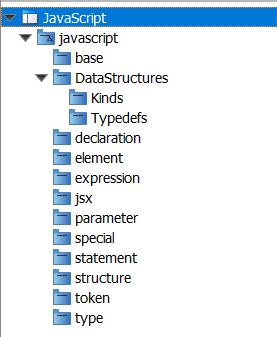
\includegraphics[width=0.4\textwidth]{JavaScriptSchema_struktura.png}
\end{figure}

\Aref{fig:JavaScriptSchema_struktura} ábrán a következő struktúra figyelhető meg: ProjektNév/Model/Packagek.
A projekt neve a JavaScript, ezen belül található egy model, amit javascript-nek hívnak. A modellen belül találhatóak meg a packagek.
A Packagek nem véletlenül így lettek elnevezve. Az alábbi hivatkozáson található meg, hogy milyen logika alapján neveztük el a packageket:~\cite{typescript-eslint}
Nem feltétlenül muszáj több packaget létrehozni, ez csupán az átláthatóság és a könnyen bővíthetőség céljából lett így megvalósítva.
Követtük a typescript-eslint githubon lévő projekt struktúrális logikáját, de több helyen is eltértünk tőle, mivel a mi projektünk másabb, illetve speciális megoldásokat igényelt egyes helyeken.
A következő oldalakon bemutatom a packagek felépítését néhány egyszerűbb példán szemléltetve.
A packagek a következőképpen épülnek fel:
\begin{figure}[!htbp]
      \caption{A base package felépítése}\label{fig:base_vpp}
      \centering
      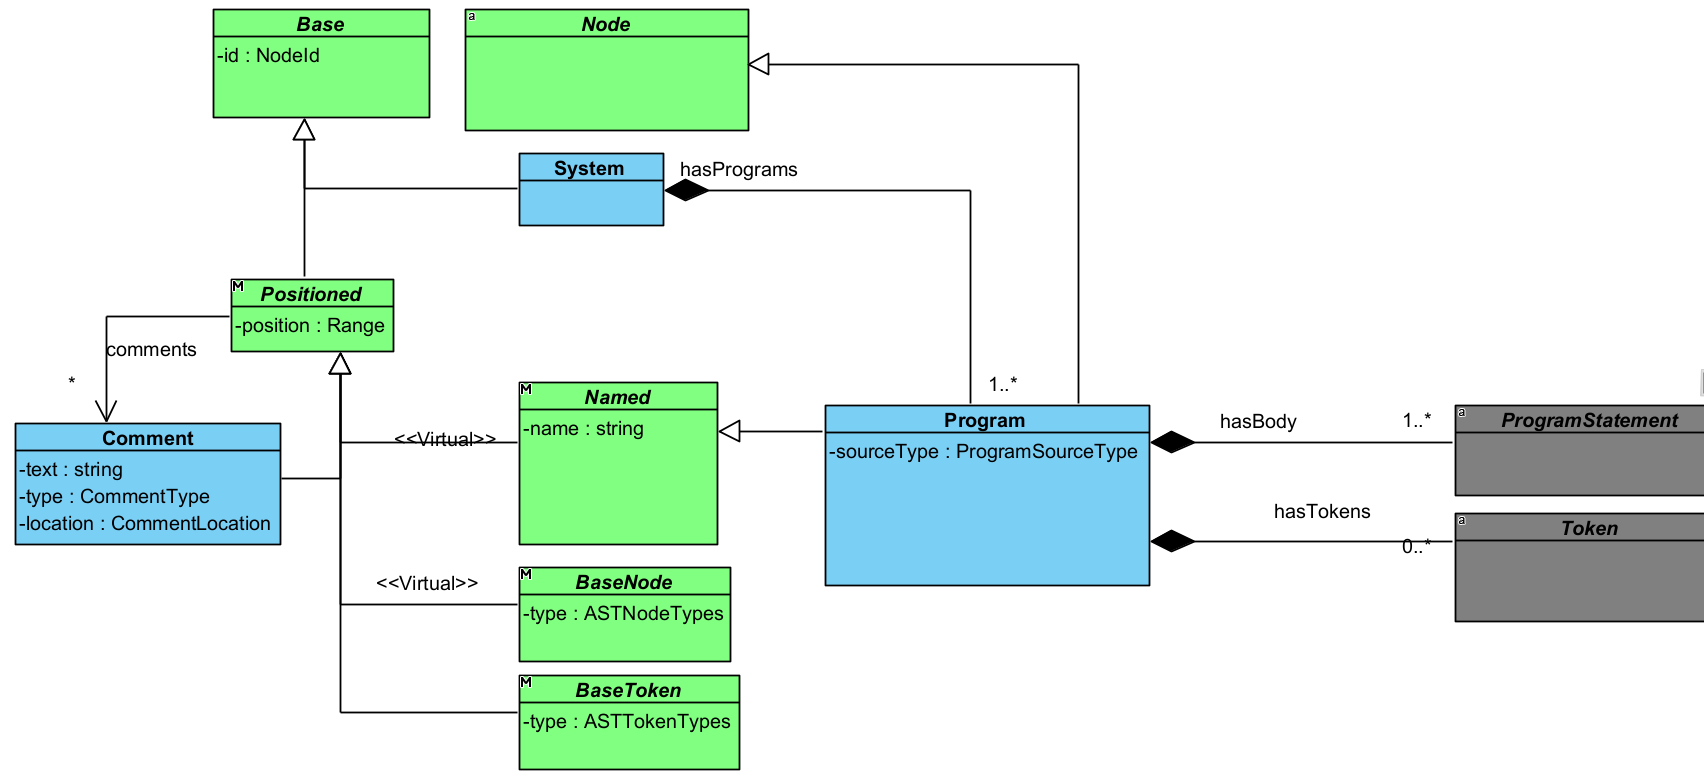
\includegraphics[width=0.9\textwidth]{base_vpp.png}
\end{figure}

\Aref{fig:base_vpp} ábrán különböző osztályok láthatóak. A Base osztály mindennek az alapja, ebből öröklődik minden más.
Látható, hogy egy id attribútummal rendelkezik, aminek a típusa NodeId.
A zöld háttérszínű osztályok az absztrakciót jelentik. Az asg fileban jelentősége, illetve a schéma szerkeszthetősége és olvashatósága miatt van így jelezve.
A szürke háttérszínű osztályok pedig csupán annyit jelentenek, hogy más packageben lettek definiálva.
A kék a default, normális osztályt jelölik.
A Positioned és a System származik le a Baseből, értelemszerűen a system az maga a program lesz.
A Positioned az azért absztrakt, mivel majd ebből fognak leszármazni a kisebb osztályok, mint például az expression, statement és a többi.
A Positioned osztálynak van egy attribútuma, a poisition, ami egy Range típus. Emellett még tartozhatnak hozzá kommentek is.
A komment egyaránt leszármazik a positioned-ből, ezzel garantálva azt, hogy a kommentnek van pozíciója.
Látható, hogy a kommentnek van egy text, type és location attribútuma. A CommentType és a CommentLocation a DataStructures-ben van definiálva.
Emellett a Named, BaseNode és a BaseToken származik le a Positionedből. A Named osztály azt jelenti, hogy egy nodenak van-e name attribútuma vagy sem.
A BaseNodeból és a BaseTokenből fog nagyon sok minden leszármazni aminek van typeja.
Végül, megtalálható a Program osztály, aminek van name attribútuma, mivel Named-ből származik le, és van Systeme. Az 1..* jelenti azt, hogy legalább 1 Systeme van, de lehet több is.
A hasPrograms-nak majd máshol lesz jelentősége, a mi esetünkben majd a javascriptben.
Tetszőlegesen el lehet nevezni, de konzisztencia miatt, minden attribútum ami osztály (és nem a DataStructuresben azon belül is a Kindsban van definiálva, hanem van neki egy osztály, mint pl Comment)
azt a hasOsztály névvel fogjuk ellátni.
A ProgramSourceType is a Kinds packageben van definiálva, ami csupán azt mondja meg, hogy az adott program vagy script vagy module típusú.
A base package nem követi a typescript-eslint githubon lévő projekt base mappáját, ez teljesen egyedi, átememeltük az egészet apróbb módosítással az előző projekt verzióból.

\noindent

A base packagen kívül bemutatom a declaration packaget, hogy lássuk milyen logikát követtünk a megírás során.
Ezen belül is az ExportAllDeclaration bemutatása:

\Aref{lst:ExportAllDeclaration} kódrészlet így lett megvalósítva a JavaScriptSchémában:
\begin{lstlisting}[caption={ExportAllDeclaration typescriptes megvalósítása},label={lst:ExportAllDeclaration}, language={JavaScript}]
export interface ExportAllDeclaration extends BaseNode {
      type: AST_NODE_TYPES.ExportAllDeclaration;
      assertions: ImportAttribute[];
      exported: Identifier | null;
      exportKind: ExportKind;
      source: StringLiteral;
}
\end{lstlisting}

\begin{figure}[!htbp]
      \caption{A declaration package felépítése}\label{fig:declaration_vpp}
      \centering
      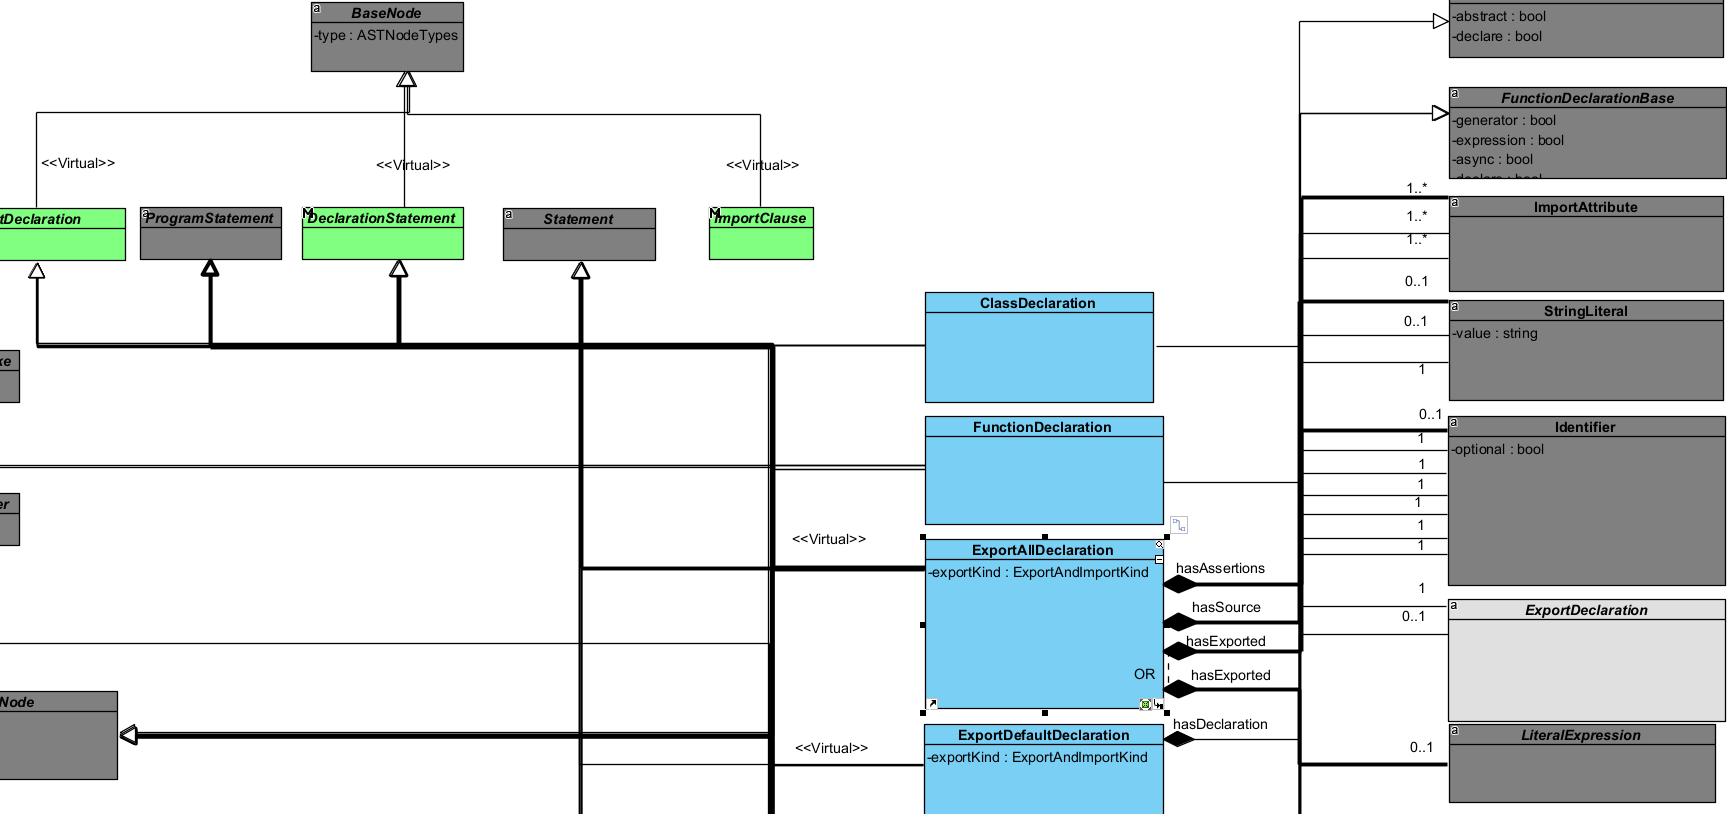
\includegraphics[width=0.8\textwidth]{declaration.png}
\end{figure}

\Aref{fig:declaration_vpp} ábrán látható az, hogy minden a BaseNodeból származik. \Aref{lst:ExportAllDeclaration} kódrészletben ez az extends BaseNode.
Itt maga a declaration osztály az a DeclarationStatement névre hallgat, csupán azért, mert követtük a typescriptes kódot. A főbb osztályok a BaseNode alatt találhatóak.
Jobb oldalt a sötétszürke és a világosszürke osztályok azok az attribútumok.
Ebben az esetben az ExportAllDeclaration osztály leimplementálását mutatom be a JavaScriptSchemában.
Az ExportAllDeclaration öröklődik a Statement, DeclarationStatement, Node és a ProgramStatementből.
Ezeket az öröklődéseket ugyanúgy a typescript-eslint githubról néztük, unions mappában találhatóak el.
Ezáltal megkapja az összes szülőnek a tulajdonságait. A DeclarationStatement öröklődik a BaseNodeból, ami azt jelenti, hogy a BaseNode tulajdonságait is megkapja az ExportAllDeclaration.
A BaseNode ugye meg származik a Positionedből, ez látható \aref{fig:base_vpp} ábrán.
Emiatt az ExportAllDeclaration-nek lesz pozíciója, kommentje és NodeId-ja is.
Assertions attribútum típusa az ImportAttribute, látható, hogy egy tömböt vár, ezért 1..* a multiplicityje.
Exported attribútumnál egy Identifier típusú attribútumot vár, itt mi kiegészítettük még egy LiteralExpressiönnel is, ami maga a Literal.
A vagyolást egy OR-al jeleztük a JavaScriptSchemában.
Mivel lehet null-is, ezért 0..1 a multiplicity, szóval vagy 0 vagy 1.
Az ExportKind az a Kindsban található meg, így szimplán csak arra hivatkozunk, mint ExportAndImportKind.
Végül a source attribútuma egy StringLiteral, nálunk is így szerepel.
Természetesen ami sötétszürkével van jelölve, az máshol létre van hozva és vannak neki attribútumai.
A világosszürke annyit jelöl, hogy ebben a packageben lett létrehozva az osztály, de láthatóság szempontból többször szerepel, mivel lehet attribútum is.
Így lett minden egyes osztály felépítve, természetesen \Aref{fig:declaration_vpp} ábra csak egy részlete a declaration packagenek, ennél jóval nagyobb.
Vannak úgynevezett gyűjtő osztályok is, mint pl a Statement, ezekre azért van szükség, mert majd később ha le lett generálva minden, akkor tudjunk majd vizsgálni különböző nodeokra, mint például az isStatement.

\noindent

Sokat említettem a DataStructurest. Hadd mutassam be egy példán keresztül, hogy ez hogy néz ki.

\begin{figure}[!htbp]
      \caption{A DataStructures packageben a Kind package felépítése}\label{fig:data_structures_kinds}
      \centering
      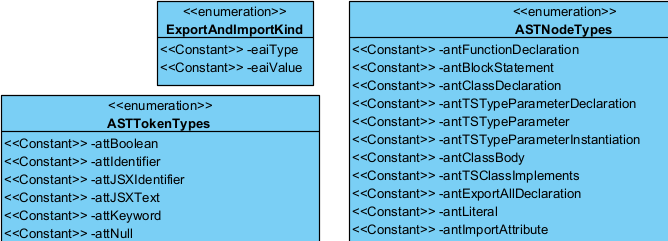
\includegraphics[width=0.8\textwidth]{data_structures.png}
\end{figure}

A DataStructures packageben található 2 package, ez \aref{fig:JavaScriptSchema_struktura} ábrán látható. Ebből a Kinds packaget mutatom be.
\Aref{fig:data_structures_kinds} ábrán látható egy kis szelet a Kinds packageből.
Enumok találhatóak ebben a packageben.
Például ha az ExportAndImportKind-ot adjuk meg típusnak az egyik attribútumnak, akkor az lehet vagy eaiType vagy eaiValue.
Minden constant előtt van 3 karakter, ez azért szükséges, mert később ezekkel még foglalkozni fogunk.

\noindent

A JavaScriptSchema magában még semmit sem csinál. Először ki kell exportálni az egész projectet xml formátumba.
Ezután az xml filet átkonvertáljuk egy asg filera. Ez úgy történik, hogy a JavaScript Analyzer projektnek van egy kisebb alprojektje, amit UmlToAsg-nek hívnak.
Ez a java kód átkonvertálja az xml fileban lévő adatot egy asg fileba. Jobban nem térnék ki az UmlToAsg projektre, mivel nem szerkesztettük.
Az UmlToAsg projektet a SchemaGenerator generálta le. A SchemaGenerator c++ nyelven megírt program. Több mindent is generál c, c++, vagy java nyelven.
Ez a projekt is az Analyzer JavaScript  alprojektei közé tartozik.
A file elején a következő található meg:
\begin{lstlisting}[caption={Asg file első sorai},label={lst:asg_file_eleje}, language={JavaScript}]
NAME = javascript;
APIVERSION = 0.3.1;
BINARYVERSION = 0.3.1;
CSIHEADERTEXT = JavaScriptLanguage;
\end{lstlisting}

A verziókat kézzel tudjuk átírni abban a fileban ami generálja ezt, ez egy c++ file, a SchemaGeneratorban található meg.
Ezután a Kinds mappa tartalmát írja bele a következőképpen:
\begin{lstlisting}[caption={Asg file kind},label={lst:asg_file_kinds}, language={JavaScript}]
KIND ASTNodeTypes (ant) {
      FunctionDeclaration;
      BlockStatement;
      ClassDeclaration;}
\end{lstlisting}
Az a 3 karakter amit minden constant elé tettünk azt kitette paraméterbe és csak az utáni stringet írta át. Ugyanígy van a többi kindnál is.
Ha az összes kindot beleírta, akkor kezdi írni sorban a többi packaget. \Aref{fig:JavaScriptSchema_struktura} alapján megy sorba.
Példának a declaration packaget mutatom be, azon belül is az ExportAllDeclaration-t.
\begin{lstlisting}[caption={Asg file ExportAllDeclaration},label={lst:asg_file_export_all_declaration}, language={JavaScript}]
SCOPE declaration {

      NODE DeclarationStatement : virtual base::BaseNode [ABSTRACT] {
      }

      NODE ExportAllDeclaration : DeclarationStatement, statement::Statement, virtual statement::ProgramStatement, special::Node {
            ATTR ExportAndImportKind exportKind;
            EDGE TREE 1 hasExported (expression::Identifier | expression::LiteralExpression);
            EDGE TREE 1 hasSource (structure::StringLiteral);
            EDGE TREE * hasAssertions (special::ImportAttribute);
      }
}
\end{lstlisting}
Látható, hogy a Packaget SCOPE-nak értelmezi, és ezen belül NODE-ok találhatóak.
A Nodeoknak ATTR és EDGE TREE van. A vagyolás is látható.
Az öröklődik egy kettőspont után, felsorolás szerűen írta át, ha valami másból származik, akkor packageNev::osztalyNev szerint.
Az kapott ATTR jelölést ami a Kinds-ban megtalálható vagy egy szimpla típus (mint pl string, int).
Minden mást EDGE TREE-nek nevezett el. Az Edge tree utáni szám vagy csillag az a multiplicitást jelenti.
Ha 1es, akkor a multiplicitás 0..1, ha *, akkor vagy 0..* vagy 1..* a multiplicitás.
\Aref{fig:declaration_vpp}as ábrán látható, hogy mit hogyan írt át.

\section{JavaScriptSchema átírása}

\noindent

A JSAN a JavaScriptSchemára épül. Ha valamit meg akarunk változtatni gyökerestül a JSANba, akkor a schémát is változtatni kell.
Azt elérni, hogy javascript mellett még typescriptes kódokat is elemezzen a JSAN, ahhoz gyökerestül meg kellett változtatni a JavaScript Analyzert.
Az előző JavaScriptSchema (ami csak javascriptet elemzett) az a javascript hivatalos oldala alapján készült. Ami ábrák fentebb megtalálhatóak, azok már az átírt schémából vannak.
Több opció is volt, hogy most vagy legyen átírva a schéma, vagy legyen egy külön typescriptre is írva.
Végül rájöttünk, hogy ha van egy typescriptes schémánk, az képes javascriptet ugyanúgy elemezni ha megfelelően van lefejlesztve.
Így egy schémát fejlesztettünk le. Az előző schéma átláthatatlan volt, ezért úgy döntöttünk, hogy majdnem a nulláról újraírjuk.
Egyedül a base packaget emeltük át a régiből, BaseNode-al és BaseTokennel kibővítve (\Aref{fig:base_vpp} ábrán látható).
Emellett el kellett dönteni, hogy milyen struktúrát kövessünk, ami jól átlatható és később könnyebben bővíthető.
Végül a typescript-eslint official github alapján haladtunk. Annyi változtatással, hogy ami nekik a base mappában volt, mi arra létrehoztunk egy külön structure packaget.
Mindenhez készítettünk dokumentációt, jól érthetően leírtuk, hogy mit miért kellett csinálni.
Mivel minden is egymásra épül a typescriptes schémában, ezért nem tudtuk tesztelni minden egyes package után, hogy működik-e vagy sem.
Mint például, látható \aref{lst:asg_file_export_all_declaration} kódrészleten, hogy az ExportAllDeclaration mennyi mindenből származik le vagy mennyire sok attribútuma van.
Az ExportAllDeclaration egyik attribútuma, az assertions típusa az ImportAttribute. Ahhoz, hogy jól észrevegye az ExportAllDeclarationt az Analyzer, ahhoz jól le kellett fejleszteni az ImportAttributet.

\begin{lstlisting}[caption={ImportAttribute},label={lst:asg_file_import_attribute}, language={JavaScript}]
export interface ImportAttribute extends BaseNode {
      type: AST_NODE_TYPES.ImportAttribute;
      key: Identifier | Literal;
      value: Literal;
}
\end{lstlisting}
Ahhoz, hogy az ImportAttributet letudjuk fejleszteni a schémában, ahhoz le kell fejleszteni az Identifiert, és a Literalt.
Kicsit összetett, hogy mi minden épül egymásra. Ebből adódik a következő alfejezet mondandója is.

\section{Nehézségek, problémák}

\noindent

A schéma átírása során több nehézségbe is ütköztünk.
A legelső nehézség az a Visual Paradigm program korrekt használata volt.
Egy kisebb időbe tellett rájönni arra, hogy egy adott classnak hogyan kell megváltoztatni a háttérszínét, packagek közötti mozgást, hogyan kell egy adott classra hivatkozni ami másik packageben volt.
Ezután ami szerintem a legnagyobb nehézség volt, az az, hogy nem volt dokumentáció az előző schémához.
Mindent nekünk kellett kitalálni, hogy mit miért csináltak az előző fejlesztők. Akik ezt a schémát fejlesztették le, ők már nem foglalkoztak ezzel, és más nem nagyon mélyedt bele ebbe az egészbe azóta.
A következő nagyobb nehézség, az az volt, hogy összehozzunk egy olyan schémát ami működőképes, és az analyzer ezt tudja is használni.
Előző alfejezetben említettem, hogy egy adott classt (mint például ExportAllDeclaration) lefejlesszünk, ahhoz sok minden mást is le kell fejleszteni, amihez meg még több minden kellett.
Ebből adódóan tesztelni nagyon nem tudtunk, mivel az egésznek működnie kellett ahhoz, hogy az analyzer egyáltalán lefusson.
Mivel mi majdnem nulláról írtuk újra, ez volt a hátrány.
Amikor elérkeztünk ahhoz az állapothoz, hogy mindenre rámondjuk azt, hogy működik, akkor jött egy nagyobb probléma.
Valahol Segmentation Fault-ot kapott a program, és nem nagyon tudtuk ezt debugolni.
Több sejtésünk is volt, hogy mi lehet a baj. Emiatt az egész schémát át kellett nézni alaposan, hogy hol vétettünk hibákat.
Sok helyen voltak pontatlanságok, rossz osztályból származtattunk le, rossz típus volt megadva attribútumnak. Ezeket mind kijavítottuk, de most már más hibát kaptunk.
A JavaScript Analyzerben kiderítettük, hogy pontosan hol szállt el a program.
A Literal volt a hiba, mivel ezt nem a github alapján írtuk meg, hanem egyedi ötlettel. Előző schémában is máshogy volt megoldva.
\begin{figure}[!htbp]
      \caption{A DataStructures packageben a Kind package felépítése}\label{fig:literal}
      \centering
      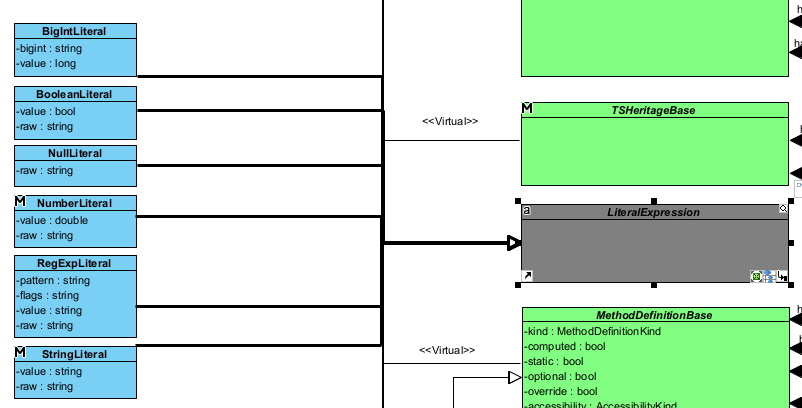
\includegraphics[width=0.8\textwidth]{literal.png}
\end{figure}

\Aref{fig:literal} ábrán látható, hogy a LiteralExpressionből (Ami a Literal) több literal is öröklődik.
\begin{lstlisting}[caption={Literal},label={lst:asg_file_literal}, language={JavaScript}]
export interface LiteralBase extends BaseNode {
  type: AST_NODE_TYPES.Literal;
  raw: string;
  value: RegExp | bigint | boolean | number | string | null;
}
\end{lstlisting}
Próbáltuk úgy megoldani, hogy 4 vagyolással 4 különböző literál tartalmazza, de az analyzerben máshogy kezeltük le a literalt, mint nodeot.
Ezért a tartalmazás helyett inkább örököltettünk a literalból, így megoldva ezt a problémát.
Még az is probléma volt, hogy volt egy LiteralBaseünk, amiből származott ez az 5 literal. A LiteralBase származott a LiteralExpressionből, de valamiért Segmentation fault lett a vége ha így próbáltuk megoldani.
Ezért a LiteralBase-t kivettük, és LiteralExpressionből származik minden literal.
Végül még az volt a nehézség, hogy kódrészletet keressünk az analyzernek, amin le tudjuk tesztelni, hogy az analyzer jó outputot ad-e.

\noindent

Mivel nem nagyon volt typescriptes háttértudásunk, először a typescriptet kellett átnézni, hogy mit hogyan tudunk megvalósítani.
Emellett még a javascriptes outputokat is át kellett nézni, mivel a mi célunk a fejlesztés volt. A jelenlegi javascriptes projektekre ugyanolyan eredményt adott, sőt néhány helyen jobbat is, mert az előző schémában is voltak pontatlanságok.
A typescriptes projektek nagy részét tudja elemezni az analyzer, de közel sem tökéletes, mivel egyfolytában kellene fejleszteni a schémát, mivel a typescript nem annyira régi.

\chapter{JavaScriptAddon}\label{chap:JavaScriptAddon}

\section{JavaScriptAddonról}

\noindent

A JavaScriptAddon az egy node kiterjesztésű file, amit a SchemaGenerator generál. Minden egyes nodenak külön generál nodeWrapperheader és egy nodeWrapperCC filet.
A SchemaGenerator által generált Factory.cc, Factory.h és az összes nodeWrapper.cc és a hozzátartozó nodeWrapper.h fileok összemergelése eredményezi a javascriptAddon.node filet.
A SchemaGenerator a JavaScriptSchemából és az ebből generált asgből generálja le a javascriptAddon.node filet.
A SchemaGeneratornak több generálása is definiálva van, hiszen nem csak erre használják. Nekünk a NodeAddonGenerator.c fileban és a hozzátartozó header fileban van minden.
A main.c-be ezt beincludeolja, és ennek hívja meg egyes metódusait, ami által elkészül a javascriptAddon.
A következő pár oldalon bemutatnám, hogy a generálás hogyan zajlik.
A SchemaGeneratornak rengeteg kapcsolója van, köztük a generateNodeAddon is. Ezekre a kapcsolókra vizsgál egyesével, egy nagy if-elseben.
\begin{lstlisting}[caption={SchemaGenerator kapcsoló vizsgálás},label={lst:schemagenerator_argv_genNodeAddon}, language={CStyle}]
else if(!strcmp(argv[i], "-genNodeAddon")){
      options.generateNodeAddon = true;
}
\end{lstlisting}
A kód elején történik meg ez, ha meg van adva paraméternek a genNodeAddon string, akkor az options.generateNodeAddon-t igazra állítja. A default értéke false.
Ezután jóval lentebb miután rengeteg mindent legenerált ami kell alapból is a normális működéshez, vizsgál egyet az options.generateNodeAddon-ra.
Ez látható \aref{lst:schemagenerator_genNodeAddon_check} kódrészleten is. Else ága nincs, szóval semmi nem történik ha nincs megadva a genNodeAddon string a paramétereknél.
\begin{lstlisting}[caption={SchemaGenerator javascriptAddon generálás},label={lst:schemagenerator_genNodeAddon_check}, language={CStyle}]
if(options.generateNodeAddon ){
      debugMessage(0, "Generating Node.JS Addon sources\n");
      if (createAndEnterDirectory(SOURCE_NODE_ADDON_DIR_NAME)) {
      generatePackageJson();
      generateBindingGyp();
      generateAddonCC();
      generateFactoryWrapper();

      if (createAndEnterDirectory("inc")) {
      generateWrapperHeaders();
      leaveDirectory();}
      if(createAndEnterDirectory("src")){
      generateWrapperSources();
      leaveDirectory();}

      leaveDirectory();}
}
\end{lstlisting}

A createAndEnterDirectory metódus annyit csinál, hogy létrehoz egy mappát és chdirrel belelép. Ha az adott mappa már létezik, akkor csak szimplán belelép.
A SOURCE $NODE\_ADDON\_DIR\_NAME$ változó jelen esetben addon értéket fog kapni, hiszen a javascriptAddon dolgai ebbe fognak generálódni.
Miután létrehozta és/vagy belelépett az addon mappába először legenerálja a package.json filet a projekthez.
A package.json fileban beállítja a projektnevét, verziószámát, dependencyket, scripteket és a végén a gypfile kapcsolónak egy true-t beállít.
\begin{lstlisting}[caption={NodeAddonGenerator package.json scripts}, label={lst:nodeAddonGenerator_package_json}, language={CStyle}]
fprintf(f, "    \"rebuild\": \"node-gyp configure && node-gyp rebuild -j 8\",\n");
fprintf(f, "    \"install\": \"node-gyp configure && node-gyp build -j 8\"\n");
\end{lstlisting}
\Aref{lst:nodeAddonGenerator_package_json} kódrészleten látható, hogy majd gyp segítségével fog történni a generálás.

\noindent

Ezután legenerálja a binding.gyp filet.
Ez a file fog felelni azért, hogy a javascriptAddonhoz sikeresen generálódjanak le a wrapperek és azok headerjei. Ha ez megtörtént, utána fogja legenerálni az addonCC-t.
Az addon.cc fileban beimportálja a Factory.h headert, amiben több metódus is megtalálható.
\begin{lstlisting}[caption={Addon.cc Wrapperek includolása}, label={lst:addoncc_wrapper_include}, language{CStyle}]
if (!traversalDescendantBFT(rootNode, generateWrapIncludes, false)) {
      debugMessage(0, " failed\n");
      fclose(f);
      return false;
}
\end{lstlisting}

\Aref{lst:addoncc_wrapper_include} kódrészletben a traversalDescendantBFT metódust egy másik projektből includoltuk.
Ez egy bejárás, ami az összes nodera lefut, és az összes nodera meghív egy metódust, jelen esetben a generateWrapIncludes metódust.
Ez a generateWrapIncludes a nodeAddonGenerator.c fileban van leimplementálva a következőképp:
\begin{lstlisting}[caption={generateWrapIncludes leimplementálása}, label={lst:addoncc_wrapper_includes_implementation}, language{CStyle}]
if(node->type.abstract){
      return true;
}
fprintf(f, "#include \"");
fprintf(f, "inc/%sWrapper.h\"\n", node->name );
return true;
\end{lstlisting}
Először megvizsgálja, hogy az adott node abstract-e, ha nem akkor tovább megy, és az addon.cc-be includolja az adott nodeWrappernek a headerjét.
A node->name lehet például FunctionDeclaration, ClassDeclaration, amik megtalálhatóak az asg fileban.

Ezután ezt a bejárást mégegyszer végrehajtja, de most a wrapperIniteket generálja az addon.cc fileba.
Annyi változtatással, hogy picit mást ír az addon.cc fileba.
\begin{lstlisting}[caption={generateWrapInit leimplementálása}, label={lst:addoncc_wrapper_inits_implementation}, language={CStyle}]
fprintf(f, "  columbus::%s::asg::addon::%sWrapper::Init(env, exports);\n", schemaName, node->name);
\end{lstlisting}

Ha ezek megtörténtek, akkor az addon.cc filet legeneráltuk sikeresen, és így benne találhatóak a wrapperek headerjének includolása és a wrapperek Initjei.

\noindent

Ezután következik egy generateFactoryWrapper hívás.
A generateFactoryWrapperben 2 metódus hivás található, a generateFactoryWrapperHeader és generateFactoryWrapperSource.

\noindent

A generateFactoryWrapperHeader a Factory.h filet generálta le a következőképp:
Először beincludolja az összes nodeWrappernek a headerjét, és utána létrehoz egy Factory osztályt, publikus metódusait, ami Init és Destructor, illetve a private metódusait,
ami a destructor, New, SaveAST, LoadAST, Clear, getRoot és az összes nodeWrapper create metódusa.
Erre azért van szükség, mivel majd a JSAN-ban ezeket a wrappereket fogjuk létrehozni és szerkeszteni.

\noindent

A generateFactoryWrapperSource pedig a Factory.cc filet generálja le.
Ebben a fileban pedig meg van az összes metódus valósítva, ami a headerjében található.
Emellett a Factory Initjének a props változója a következőképpen néz ki:
\begin{lstlisting}[caption={Factory.cc file}, label={factory_cc}, language={CStyle}]
napi_property_descriptor props [] = {
      DECLARE_NAPI_METHOD("getRoot", getRoot),
      DECLARE_NAPI_METHOD("createCommentWrapper", createCommentWrapper)
      ...}
\end{lstlisting}

DeclareNapiMethodokat hoz létre, az összes nodeWrappernek, ezek majd a JSAN-ban lesznek használatosak.

\noindent

Utolsó lépésként, először az inc mappát majd az src mappát generálja le a SchemaGenerator.
Az inc mappában találhatóak a header fileok egyes wrappereknek, az src mappában maguk a wrapperek vannak megvalósítva.
Minden nodenak hoz létre wrapper filet, és ezekben valósít meg néhány metódust.
Vegyük most egy példának az ExportAllDeclarationt. Létrehoz egy ExportAllDeclarationWrapper.h és egy ExportAllDeclaration.cc filet.
A header fileban létrehoz egy ExportAllDeclarationWrapper osztályt, ami származik a BaseWrapperből. A BaseWrapper az egy alap Wrapper osztály, amit bővíteni fogunk.
Három publikos metódust generál, Init, Destructor és a NewInstancet.
Ezen felül több private metódust is.
\begin{lstlisting}[caption={ExportAllDeclaration.h file}, label={lst:ExportAllDeclaration_header}, language={CStyle}]
napi_property_descriptor props [] = {
      static napi_value setPosition(...);
      static napi_value addAssertions(...);
      static napi_value setType(...);
...}
\end{lstlisting}

Látható \aref{lst:ExportAllDeclaration_header} kódrészleten, hogy létrehozott az ExportAllDeclarationWrappernek egy setPosition, addAssertions, setType és még több metódust.
Ezek az ExportAllDeclaration attribútumai, amit a JavaScriptSchemában beállítottunk.
\Aref{fig:declaration_vpp} ábrán látható, hogy az ExportAllDeclaration hasAssertions attribútumának a multiplicitása 1..*, ezt átkonvertálta addAssertionsre.
Ahol 0..* a multiplicitás, azt átkonvertálta setAttribute-ra, pl setSource vagy setExportedre.
Minden nodeWrappernek van olyan metódusa, hogy setPath, setPosition, setType, addComments, hiszen minden a BaseNode vagy a BaseTokenből öröklődik le.

\noindent

Az ExportAllDeclaration.cc fileban ugyanaz történik, mint ami volt a Factory.cc fileban. Declare napi methodokat generál, a setExported, setSource, setType és a többi metódushoz.
Ezután az összes metódust megvalósítja.

\section{JavaScriptAddon változások}

\noindent

A JavaScriptSchema változtatások után, a NodeAddonGeneratort nem módosítottuk.
Ennek ellenére a javascriptAddon.node mérete megduplázódott, csupán azért, mert a schéma ekkora bővítésen esett át.
Sokkal több nodeWrapper lett, mivel bejöttek a typescript általi dolgok is a javascript mellett.
Természetesen a javascriptes dolgok megmaradtak, így javascriptet ugyanolyan jól tud elemezni, sőt néhány esetben jobban is, mert voltak figyelmetlenségek előző verzióban.

\noindent

Mivel a javascriptAddon mérete nőtt, ezáltal a sebesség csökkent.
Ezt majd egy másik fejezetben jobban kifejtem, célunk az volt, hogy először tudjon typescriptes fileokat és projekteket elemezni a jsan.

\chapter{JSAN2Lim átírása}\label{chap:JSAN2Lim átírása}
-halstead, stb
-miben kellett bőviteni, mi hiányzott
-mit nem detektált
\section{JSAN2Limről}

\section{Bővítések}

\section{Miket nem detektált}

\chapter{AST Binder Optimalizálás}\label{chap:AST Binder Optimalizálás}

\section{A binderről}

\noindent

Az AST binder referenciákat bindol. Ezek a referenciák a JSAN2Lim programhoz kellenek.
Binder néven van definiálva az astTransformer.js fileban.
Kétszer van használva, ezért is kulcsfontosságú, hogy gyors legyen.
Egyszer VariableUsages referenciákat bindol és egyszer ACG referenciákat bindol.
\noindent

A binder 4 argumentumot vár:
\begin{itemize}
      \item Egy stringet, ami lehet vagy VU (ami VariableUsages-t rövidíti) vagy ACG (egy javascript callgraph).
      \item Egy Abstract Syntax Tree-t (AST), ami egyedien van felépítve.
      \item Egy tömböt, amiben JSON objektumok találhatóak, amik a linkeket tartalmazzák.
      \item Végül még egy stringet, ami lehet addCalls, vagy setRefersTo. Az AddCalls és a SetRefersTo a javascriptAddonban található meg. Akkor addCalls ha ACG referenciákat bindolunk és akkor setRefersTo ha VU referenciákat.
\end{itemize}

Egy JSON objektum a következőképp néz ki:
\begin{lstlisting}[caption={Binder JSON argumentuma}, label={lst:binder_json_arg}, language={JavaScript}]
source: {
      label: IdentifierNeve,
      file: AbsPath,
      start: { row: <int>, column: <int>},
      end: { row: <int>, column: <int>},
      range: { start: <int>, end: <int>},
      node: [Object]
},
target: {...}
\end{lstlisting}

\noindent

\Aref{lst:binder_json_arg} kódrészletben egy JSON elemét láthatjuk a tömbnek. Ilyen JSON elemekből épül fel a tömb.
A source és a target felépítése ugyanaz, csupán másak az értékek bennük.
A kódrészletben csak a sourcet fejtettem ki kicsit bővebben. A label az egy Identifiert vagy PrivateIdentifiert fog jelölni.
A file egy abszolút útvonalat, ami az Identifiert tartalmazó filet jelöli.
A start az egy object, amiben külön van sor és oszlop meghatározva. Ez az Identifier első karakter pozíciójának a sor és oszlop értékei.
Az end ugyanaz, mint a start, csak itt az utolsó karakter pozíciójának a sor és oszlop értékei.
A range is egy object, a start ennél a kezdő karakter hanyadik karakter volt a kódban, és az end pedig az identifier utolsó karakterének a karakterszáma.
A node is egy object.

\section{Lassúság okai}

A binder nagyobb projektekre nagyon lassan fut le. Ennek több oka is van:
\begin{itemize}
      \item Minden hívásnál meghívja a javascriptAddon.nodeot, ami már magában nagy file. TypeScript támogatás után kétszeres lett a mérete, ezáltal sokkal lassabb lett.
      \item Mivel nagyobb a projekt, ezért sokkal több a függvény hívás is az elemzett kódban, emellett sok a változószám is.
      \item Az AST nagyon nagy, és ezt bejárjuk többször is bindolás alatt. Emiatt nagyon lassú a program nagy projektek esetén.
      \item A JSON objektum is nagyon nagy lesz, de annyira ez nem lassítja le a programot.
\end{itemize}

\section{Optimalizálás}

\noindent

Először ki kellett derítenem, pontosan melyik funkció mennyi memóriát vesz igénybe és milyen gyorsan fut le.
Erre találtam egy javasript profilert, ami kiírta minden függvén hívásnál a memóriafoglalást.
Ez nekem nem volt a legjobb, mivel nagyon egybe van ágyazva minden, és eléggé mélyre mentek a functionok.
Ezután próbáltam picit egyszerűbbet, a binder kódját 3 részre osztani, console.time és console.timeEnd használatával.
Így megkaptam, hogy melyik rész nagyjából mennyi idő alatt fut le, könnyebb volt szűkíteni, hogy melyik function lesz a bajos.
Végül kiderült, hogy a következő sor lassítja be nagyon a programot:
\begin{lstlisting}[caption={Problémás function}, label={lst:binder_problemas_function}, language={JavaScript}]
globals.getWrapperOfNode(resolveNode(astSet, sourceFile, element.source.range.start, element.source.range.end, true));
\end{lstlisting}

Ezen belül is a resolveNode function volt a probléma, mivel a resolveNode kapott egy AST-t (amit a binder kapott meg paraméterbe), egy filenevet, kezdő és vég paramétert, illetve egy true vagy falset, attól függ, hogy sourcenodeot vagy targetnodeot keresünk.
Az AST-n forEach-el végigmentünk, amin belül walk-al bejártuk addig amíg nem találtuk meg a számunkra kellő filet.
Kisebb projekt esetében ez nem baj, mivel az AST nem annyira nagy. Ahol már van 100 vagy 200 ezer változó és vagy függvény hívás, ott már nagy gondok lehetnek, mivel ezt rengetegszer meg kell ismételni, ami iszonyat lassú.
Nem elég ezt egyszer megtenni, kétszer kell, mivel ezt a VU-ra és az ACG-re is végre kellett hajtani.

\noindent

Így már tudtam, hogy mit kell átírni, vagy átgondolni, hogy hogyan lehetne ezt a többszöri bejárást csak egyszer végrehajtani, és az adott tömbből adatokat kinyerni.
%getIndexed --> ugyanolyan paraméterek, mint a resolveNodenál, kivéve annyival, hogy nem kap ast-t.
% Tömbbe tesszük be, picit jobban kifejteni, hogy mit miért. JavaScript profilerről szót ejteni, hogyan derítettem ki, hogy mi használ sok memóriát és lassú
\section{Eredmény}
% 5-10x gyorsulás nagyobb projekteken, ide majd egy képet, hogy before/after egy adott projektre, kevesebb memória igény

\chapter{Regressziós tesztek frissítése}\label{chap:Regteszt_frissítés}

\section{Tesztek kibővítése}
Először kezdtem a JSAN tesztek átírásával. A JSAN-nak a következő kapcsolói voltak:
\begin{itemize}
      \item -i: Jelentése input, lehet relatív vagy abszolút útvonal a fáljoz vagy projekthez.
      \item -o: Jelentése output neve, lehet relatív vagy abszolút útvonal.
      \item -d: Jelentése dumpjsml, a JSAN eredményét átgenerálja XML stílusú fájlba és ezt egy jsml fájlba kiírja.
      \item -e: Jelentése ExternalHardFilter, relatív vagy abszolút útvonal egy olyan fájlhoz, ami szövegalapú és olyan szintaxis található benne, ami kell az externalHardFilternek.
      \item -help: Kiírja minden kapcsolóhoz tartozó leírást.
      \item -r: Jelentése useRelativePath, eredményben az útvonalakat átírja relatív útvonalra.
      \item -h: Jelentése html, a JSAN html fájlokra is lefut, bennük keresve JavaScript-es szkripteket és azokat teszteli.
      \item -stat: Jelentése statistics, kiírja a memóriahasználatot és a futásidőt amit a JSAN vett igénybe.
\end{itemize}


Az input, output, dumpjsml, ExternalHardFilter, és html kapcsolókra tudtam tesztelést írni. A logika az volt, hogy mappanév alapján tesztelek egyes kapcsolókra.
ProgramozásiNyelv-kapcsolónév logikát követtem, mivel JavaScript-es tesztek mellé kell majd TypeScript-es teszteket is keresnem.
A projekteket python szkriptek segítségével futtattam le.

\begin{lstlisting}[caption={JSAN kapcsoló vizsgálat pythonban}, label={lst:python_kapcsolo}, language={Python}]
if "externalHardFilter" in input_path:
      ret_val = self._execute_one_test(input_path, external_hard_filter=True) and ret_val
      return ret_val
\end{lstlisting}

\Aref{lst:python_kapcsolo}-es kódrészleten látható, hogy hogyan keresek egy adott kapcsolóra. Az input\_path-ban van a mappa is, és a js-externalHardFilter-ben megtalálható az externalHardFilter szó.
Az execute\_one\_test függvényemben beállítom a teszteléshez az adott dolgokat.

\begin{lstlisting}[caption={JSAN kapcsoló beállítása pythonban}, label={lst:python_kapcsolo_beallitasa}, language={Python}]
if external_hard_filter:
      input_dir = os.path.dirname(input_path)
      external_hard_filter_path = os.path.join(input_dir, "externalHardFilter.txt")
      external_hard_filter_switch = "-e"
else:
      external_hard_filter_path = ""
      external_hard_filter_switch = ""
\end{lstlisting}

\Aref{lst:python_kapcsolo_beallitasa}-es kódrészletben az execute\_one\_test függvénynek egy részét láthatjuk, ahol beállítjuk az external\_hard\_filter\_path-t és a kapcsolót annak függvényében, hogy igazat kaptunk e vagy sem.
Létrehozzuk az externalHardFilter fájlt a tesztelendő fájl mellé vagy a tesztelendő projekt gyökerébe,
és attól függően, hogy ki akarjuk hagyni az adott fájlt vagy hozzáadni, írunk egy $+$ vagy egy $-$ jelet a sor elejére és utána relatív útvonal és a fájl neve.
Alapértelmezetten minden fájl elemez az adott program, JSAN esetében ezek azok a fájlok amiknek a kiterjesztése \texttt{js}, \texttt{jsx}. (külön kapcsolóval megadhatjuk neki, hogy a html kiterjesztésű fájlokat elemezze-e vagy se.)
TypeScript-es bővítés után már a ts és a tsx kiterjesztésű fájlokat is elemzi. Ezért írtam több tesztesetet is. Egy példa, hogy hogyan néz ki ez a fájl:

\begin{lstlisting}[caption={ExternalHardFilter fájl}, label={lst:external_hard_filter}]
-filtered01
-filtered02
-filtered03
+filtered01
\end{lstlisting}

\Aref{lst:external_hard_filter}-as kódrészletben látható, hogy filtered01, filtered02 és filtered03 at kivettük, hogy azokat ne elemezze a jsan.
Ezután visszavettük a filtered01-et. A filtered fájlok azok JavaScript-es fájlok, JavaScript-es kóddal.
Ezután referenciába csak a filtered01 fájl eredményét raktam be, hiszen a 02 és 03-at nem elemzi, ha elemezné, akkor szólna a program, hogy hiányzó referecia fájl.
Természetesen lehet regurális kifejezést is használni filterezésnél.


Ezután teszteltem a \texttt{-i} kapcsolót, itt a programnak vissza kellene adnia, hogy üres az input ha nincs megadva.
Ezután a \texttt{-o} kapcsolóra teszteltem, itt ebben az esetben alapértelmezett értékben \texttt{out.jssi} fájlt kellene visszaadnia.
Végül a \texttt{-h} kapcsolót néztem meg, itt ha megvan adva ez a kapcsoló, akkor az adott projektben a html fájlokban a JavaScript-et kellene tesztelni.
A \texttt{-d}, \texttt{-help}, \texttt{-stat} kapcsolókra nem tudtam tesztelni, még a \texttt{-useRelativePath} kapcsolóra sem, hiszen ha abszolút utat kérek, akkor a referenciákban másnál rossz lesz az elvárt eredmény.


Ezután a JSAN2Lim és az ESLintrunner programoknak írtam át a tesztelési menetetét, mivel nekik volt még olyan kapcsoló, amit lehetett tesztelni. A többi projektnek 1 vagy 2 volt, amik kellettek a működésükhöz, nem voltak opcionális kapcsolók.

Miután a JSAN ki lett egészítve TypeScript támogatással és a JSAN2Limet átírtam, elkezdtem teszteket keresni, mind a JSAN-nak és mind JSAN2Lim-nek.
Kerestem egyszerűbb TypeScript és picit összetettebb TypeScript projekteket is, hogy lássam az esetleges hiányosságokat.
Természetesen ami eredményeket adtak a programok, azokat át kellett néznem egyesével, hiszen csak így tudom meg, hogy jól tesztelte-e a megadott fájlt vagy sem.
Több kisebb hiányosságot is észrevettem, mind JSAN oldalról, mind JSAN2Lim oldalról, ezek kisebb hiányosságok voltak.
Például, hogy egy node-nak nem volt beállítva pozíció, vagy nem volt jól beállítva a paramétere.

\chapter{Összefoglaló}\label{chap:Összefoglaló}

\section{Program javulása}

\noindent

A szakdolgozatom során sikerült elérnem azt, hogy az Ast binder közel tízszer gyorsabban fusson le nagyobb projektre, mint ezelőtt.
Leteszteltem ugyanarra a nagy projektre az eredeti JSAN lefutását és az én általam átírt lefutását. Ezt \Aref{lst:jsan_before_after_comparison} kódrészleten láthatjuk.
Kisebb projektekre körülbelül ötszörös gyorsulás van.
Lefuttattam egy nagyobb projektre a jsan-t, az optimalizált és az optimalizálatlan verzióval, hogy jobban lássuk a különbséget. A következő eredmények születtek:

\begin{lstlisting}[caption={JSAN lefutási idő előtte és utána}, label={lst:jsan_before_after_comparison}]
Optimalizalt_verzio:
Binding VU: 71599/71599
VU binding: 1:39.140 (m:ss.mmm)

Optimalizalatlan_verzio:
Binding VU: 71599/71599
VU binding: 42:31.211 (m:ss.mmm)
\end{lstlisting}

Ugyanazt az outputot adja mind a kettő program, szóval csak gyorsaságban és memóriahasználatban változott sokat.

Emellett a JavaScriptSchema újraírása is sikeres volt, emiatt a JSAN tud typescriptes kódokat elemezni.
JSAN2Limet sikeresen módosítottam, hogy a JSAN által kiadott outputot sikeresen limmé alakítsa.
\section{Jövőbeli tervek}

\noindent

JavaScriptSchema bővítése sok időbe telt, mivel se dokumentáció, se tapasztalat nem volt. Ezután még a JSAN2Lim átírás is sok időbe került.
Eközben a typescript-eslint github repo amit használtunk a bővítésre, frissült, sok új funkciót hoztak be.
Rengeteg változtatás volt a typescript résznél, de a schémát nem tudtuk még naprakészre hozni, mivel voltak ennél fontosabb feladatok.
Egyik jövőbeli terv az, hogy a schémát up to datere hozzam, mivel már van hozzá dokumentáció is, meg nagyjából én is írtam, ezért nem lesz ez annyi idő, mint volt az elején az újraírása.

\noindent

Végül a JSAN programra még bőven ráfér az optimalizálás, mivel csak az ast bindert optimalizáltuk, rengeteg helyen feleslegesen van bejárva az ast.
Ez a másik jövőbeli terv.

\include{tex/Nyilatkozat}
\addcontentsline{toc}{chapter}{Köszönetnyílvánítás}
\chapter*{Köszönetnyílvánítás}

\addcontentsline{toc}{chapter}{Irodalomjegyzék}
\bibliographystyle{plain}
\bibliography{references}

\end{document}
